\documentclass[conference]{IEEEtran}
% newtx gives real Times metrics under both XeTeX (tectonic, local
% builds) and pdfLaTeX (arXiv), so both variants typeset identically.
\usepackage{newtxtext,newtxmath}
\usepackage{microtype}
\emergencystretch=1em
\usepackage{graphicx}
\usepackage{booktabs}
\usepackage{amsmath}
\usepackage[hidelinks,pdfauthor={},pdfcreator={},pdfproducer={}]{hyperref}
% AUTO-GENERATED by scripts/check_paper_numbers.py -- do not edit.
% Single source of truth for data-derived numerals.
\newcommand{\NumBatteryLo}{-0.7}
\newcommand{\NumBatteryHi}{4.5}
\newcommand{\NumSevenLo}{-0.8}
\newcommand{\NumSevenHi}{5.2}
\newcommand{\NumHeadroomLo}{-2.0}
\newcommand{\NumHeadroomHi}{7.1}
\newcommand{\NumHardLo}{-16.1}
\newcommand{\NumHardHi}{12.9}
\newcommand{\NumHeadroomDisc}{11.7}
\newcommand{\NumHardDisc}{31.7}
\newcommand{\NumCensusPairs}{79}
\newcommand{\NumCensusEquiv}{18}
\newcommand{\NumCensusDiff}{59}
\newcommand{\NumCensusDiffKept}{57}
\newcommand{\NumCensusMedian}{8}
\newcommand{\NumCensusNoEight}{12}
\newcommand{\NumCensusWithEight}{4}
\newcommand{\NumWaldEquiv}{18}
\newcommand{\NumWaldSat}{17}
\newcommand{\NumWaldInf}{3}
\newcommand{\NumUnpEquiv}{14}
\newcommand{\NumUnpSat}{14}
\newcommand{\NumUnpInf}{0}
\newcommand{\NumSevenEquiv}{20}
\newcommand{\NumSevenInf}{10}
\newcommand{\NumSevenSat}{19}
\newcommand{\NumThreeEquiv}{3}
\newcommand{\NumStepContrasts}{21}
\newcommand{\NumStepEquiv}{11}
\newcommand{\NumStepEquivKept}{0}
\newcommand{\NumCensusEquivKept}{1}
\newcommand{\NumCensusSatKept}{17}
\newcommand{\NumAbstractAudit}{Among $86$ VLA efficiency papers claiming parity on LIBERO, $76\%$ compare against a base policy at or above $90\%$ success and $15$ report any uncertainty, per-task result, or paired analysis.}
\newcommand{\NumEffInc}{86}
\newcommand{\NumEffScreened}{354}
\newcommand{\NumEffCeil}{76}
\newcommand{\NumEffCeilNf}{66}
\newcommand{\NumEffGap}{-0.2}
\newcommand{\NumEffAny}{15}
\newcommand{\NumEffPaired}{one}
\newcommand{\NumEffNoN}{45}
\newcommand{\NumEffUsable}{47}
\newcommand{\NumEffCert}{38}
\newcommand{\NumEffCertRatio}{14}
\newcommand{\NumEffLarger}{9}
\newcommand{\NumEffPairs}{30}
\newcommand{\NumEffPlotted}{84}
\newcommand{\NumEffVerAuto}{51}
\newcommand{\NumEffVerFields}{54}
\newcommand{\NumEffVerMiss}{3}
\newcommand{\NumSeedEightLo}{-0.7}
\newcommand{\NumSeedEightHi}{4.5}
\newcommand{\NumSeedLenDiff}{59}
\newcommand{\NumRepLenDiff}{38}
\newcommand{\NumCertCells}{13}
\newcommand{\NumHolmDiff}{48}
\newcommand{\NumDiffKeptSat}{38}
\newcommand{\NumNinetyEquiv}{20}
\newcommand{\NumNinetySat}{18}
\newcommand{\NumNinetyInf}{5}
\newcommand{\NumPiZeroLo}{-12.1}
\newcommand{\NumPiZeroHi}{-3.8}
\newcommand{\NumSmolLo}{-6.2}
\newcommand{\NumSmolHi}{1.6}
\newcommand{\NumLayoutLo}{-3.0}
\newcommand{\NumLayoutHi}{4.3}
\newcommand{\NumCameraLo}{-7.3}
\newcommand{\NumCameraHi}{-2.0}
\newcommand{\NumOtherVarMax}{0.063}
\newcommand{\NumStepLatency}{1.4}
\newcommand{\NumChunkOne}{66}
\newcommand{\NumChunkTen}{94}
\newcommand{\NumSeedTaskNineA}{3--1}
\newcommand{\NumSeedTaskNineB}{7--4}
\newcommand{\NumSubsetsAboveSat}{1}
\newcommand{\NumStepDiff}{10}
\newcommand{\NumStepDiffKept}{9}
\newcommand{\NumFrBat}{0.65}
\newcommand{\NumFrBatLo}{0.31}
\newcommand{\NumFrBatHi}{1.21}
\newcommand{\NumFrInf}{0.70}
\newcommand{\NumFrInfLo}{0.30}
\newcommand{\NumFrInfHi}{1.30}
\newcommand{\NumFrCam}{1.08}
\newcommand{\NumFrCamLo}{1.03}
\newcommand{\NumFrCamHi}{1.14}
\newcommand{\NumFrPiZero}{1.53}
\newcommand{\NumFrPiZeroLo}{1.19}
\newcommand{\NumFrPiZeroHi}{1.96}
\newcommand{\NumCamHiA}{31}
\newcommand{\NumCamHiB}{74}
\newcommand{\NumCamLoA}{14}
\newcommand{\NumCamLoB}{10}
\newcommand{\NumPiZeroCost}{7.9}
\newcommand{\NumPiZeroP}{0.00025}
\newcommand{\NumCameraCost}{4.7}
\newcommand{\NumCertifyPairs}{520}
\newcommand{\NumCertifyHard}{1{,}280}
\newcommand{\NumDialSentence}{Of the $24$ audited papers whose own method uses a flow or diffusion action head, $7$ state the denoising step count used in evaluation, $6$ the execution horizon, and at most $4$ both, so the two settings whose effects Sec.~\ref{sec:transfer} measures are usually unrecoverable from the paper. }

\newif\ifanon \anontrue % set \anonfalse for arXiv/camera-ready

% Anonymized for double-anonymous review (ICRA 2027).

\title{Certified by the Ceiling: Saturated Benchmarks Supply the No-Loss Claims Behind VLA Acceleration}
% Author identity is injected at build time by scripts/build_named.sh so the
% tracked source carries none, and any anonymized mirror of this repo is safe
% regardless of its term list.
\author{\IEEEauthorblockN{\ifanon Anonymous\else AUTHORNAME\fi}
\ifanon\else\IEEEauthorblockA{AUTHORAFFIL\\AUTHOREMAIL}\fi}

\begin{document}
\maketitle

\begin{figure*}[t]
\centering
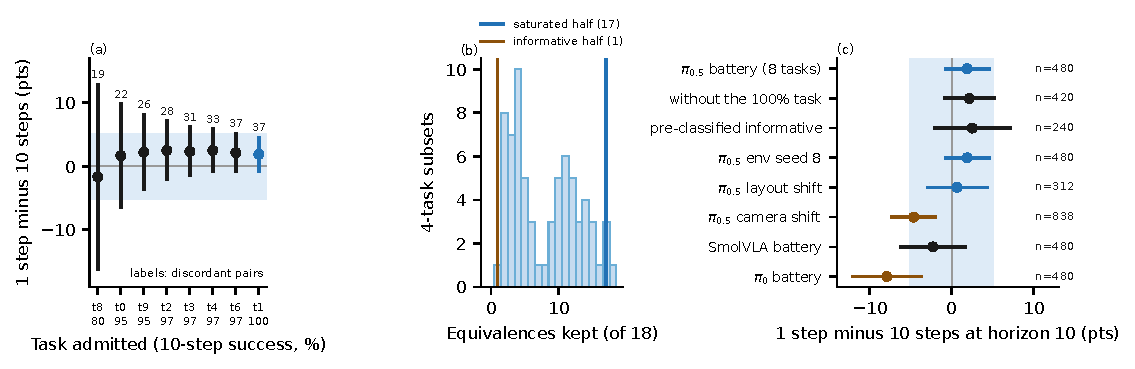
\includegraphics[width=\textwidth]{figures/fig_transfer.pdf}
\caption{Where equivalence certificates come from. All panels: one
denoising step minus ten at execution horizon 10 (SmolVLA: minus its
served default; paired Newcombe 95\% intervals; shaded band: $\pm5$-point
equivalence margin). (a)~$\pi_{0.5}$ on the LIBERO-10 battery, admitting
tasks from least to most successful under ten steps (tick labels: task,
ten-step success); labels count discordant pairs. The interval enters the
margin (blue) only after the near-saturated tasks are admitted; the last,
perfectly solved task adds $60$ pairs and no discordant one. (b)~The
$\NumCensusEquiv$ comparisons in our grids that certify equivalence on the
battery, re-tested on each of the $70$ four-task subsets ($240$ pairs
each): the saturated half keeps $\NumCensusSatKept$, the informative half
$\NumCensusEquivKept$. (c)~The same contrast where failures are common.
Brown: significant difference ($p{<}0.05$); otherwise blue: equivalent at
$\pm5$; black: inconclusive.}
\label{fig:transfer}
\end{figure*}

\begin{abstract}
Papers that make vision-language-action (VLA) policies cheaper to run
justify their speedups by showing no loss on LIBERO, where base policies
typically succeed in more than $90\%$ of episodes. We show that such no-loss
verdicts are supplied by tasks both settings already solve, and so say
little about the tasks on which policies fail. Re-testing the
best-documented case, a single denoising step on released flow-matching
checkpoints, one step is equivalent to ten within $\pm5$ points on an
eight-task LIBERO-10 battery for $\pi_{0.5}$, yet inconclusive on the four
tasks classified as informative before the experiment
($[\NumHeadroomLo, +\NumHeadroomHi]$ points). The pattern is systematic:
of $\NumCensusEquiv$ equivalence certificates among $\NumCensusPairs$
paired comparisons, the four saturated tasks keep $\NumCensusSatKept$ and
the four informative tasks keep $\NumCensusEquivKept$ at equal episode
counts, while the informative tasks keep $\NumCensusDiffKept$ of
$\NumCensusDiff$ significant differences. Where failures are common,
the verdicts diverge: one step costs $\pi_0$ $\NumPiZeroCost$ points
($p{=}\NumPiZeroP$) and $\pi_{0.5}$ $\NumCameraCost$ points under large
camera-viewpoint shifts ($p{=}0.0008$). The problem is widespread.
\NumAbstractAudit{} We propose a three-part report for no-loss claims,
show that a relative failure margin alone is lenient in the opposite
regime, and give the paired-episode budget that certification on
informative tasks requires.
\end{abstract}

\section{Introduction}
Making vision-language-action (VLA) policies cheaper at inference is now
a research area of its own: fewer denoising steps~\cite{snapflow2026,chen2026simple},
caching~\cite{oi2026actioncache}, adaptive computation~\cite{han2026adavla},
token pruning, and quantization, applied to released policies such as
$\pi_0$, $\pi_{0.5}$, and SmolVLA~\cite{black2024pi0,pi05,shukor2025smolvla,pi07}.
These papers share one form of evidence: the accelerated policy shows no
loss against its base on LIBERO~\cite{liu2023libero}, where the base
already succeeds in nearly every episode. Released $\pi_{0.5}$, for
example, loses $0.2$ points at a single denoising
step~\cite{oi2026actioncache}.\footnote{Per-episode logs for every reported number, the audit protocols and extractions, and the harness: \ifanon\url{https://anonymous.4open.science/r/flow-dials-eval}\else \url{https://github.com/nihalgunu/roborigor}\fi}

\textbf{The claim of this paper} is that such no-loss verdicts are largely
supplied by tasks both settings already solve. A pair of episodes that
both succeed is evidence that the settings agree on that episode, but it
tightens an absolute-difference interval for the pooled average while
carrying no information about the episodes where a setting could fail.
Non-inferiority trials know this failure mode as the leniency of
absolute margins at low event rates~\cite{quartagno2020,redfors2024};
saturated robot benchmarks keep evaluation permanently in that regime,
and what it does to robot-policy claims has not been measured.

We measure it on the best-documented case, a single denoising step on
released flow-matching checkpoints. The favorable result reproduces with
a formal equivalence test, but only once near-saturated tasks are
admitted (Fig.~\ref{fig:transfer}a). Across every paired comparison in
our grids, saturated tasks keep nearly all equivalence certificates and
informative tasks keep almost none, while significant differences survive
on the informative tasks (Fig.~\ref{fig:transfer}b). Where failures are
common the verdicts diverge by policy and condition
(Fig.~\ref{fig:transfer}c). An audit of $\NumEffInc$ VLA efficiency papers
shows that the field's no-loss claims sit in exactly this regime
(Fig.~\ref{fig:efficiency}).

\textbf{Why it matters.} Authors of efficiency methods, reviewers who
assess them, and practitioners who deploy them currently read ``no loss on
LIBERO'' as evidence that a speedup is free. It is evidence that the
speedup is free on tasks the policy already solves. Our reporting rule
tells each of them what to ask for instead.

\textbf{Contributions.}
(1)~We show and quantify that equivalence verdicts in VLA evaluation are
supplied by saturated tasks, with a task classification fixed before the
experiment, an equal-size control over all task subsets, and sensitivity
to interval and margin (Sec.~\ref{sec:dilution}).
(2)~We show that the VLA efficiency literature rests on such verdicts:
an audit of $\NumEffInc$ papers claiming no loss on LIBERO
(Sec.~\ref{sec:audit}).
(3)~We show what happens where failures are common, on three released
policies and two LIBERO-Plus shifts, and derive a three-part report and
the paired-episode budget for certifying no-loss claims
(Secs.~\ref{sec:dilution}, \ref{sec:transfer}).

\section{Related Work}\label{sec:related}
\textbf{Equivalence and non-inferiority testing.} Equivalence is
conventionally shown with two one-sided tests~\cite{schuirmann1987},
and reporting standards for equivalence and non-inferiority trials
require the margin to be justified~\cite{piaggio2012consort}. A margin on
the absolute risk difference becomes lenient when the reference event
rate is low, which motivates relative margins and non-inferiority
frontiers~\cite{quartagno2020,redfors2024}; paired designs call for
intervals that respect the pairing~\cite{newcombe1998paired,tango1998}.
We carry these results into robot-policy evaluation, where the event is
failure and benchmark saturation drives its rate to a few percent.

\textbf{VLA acceleration.} Single- and few-step inference for flow
VLAs has been obtained by distillation~\cite{snapflow2026}, one-step
training~\cite{chen2026simple}, caching~\cite{oi2026actioncache}, and
adaptive step counts~\cite{han2026adavla}; regression can match
generative control~\cite{pan2026noising}, and execution horizon trades
speed against reactivity~\cite{wang2026autohorizon,black2025rtc}.
ActionCache reports $\pi_{0.5}$ collapsing at one step on
VLABench~\cite{oi2026actioncache}, a far higher failure regime than
LIBERO. We do not propose an acceleration method; we test what the
evidence these methods report can establish.

\textbf{Evaluation methodology.} Seed variation can flip deep-RL
conclusions~\cite{henderson2018matters,agarwal2021precipice}, and
unreported variance inflates claimed progress in language
models~\cite{hochlehnert2025sober,miller2024errorbars}. In robotics,
paired evaluation with posterior uncertainty is practiced at scale by
the LBM study~\cite{lbm2026}, sequential tests stop comparisons
early~\cite{snyder2025step,snyder2026beyond}, best practice has been set
out~\cite{kressgazit2024empirical}, and PhAIL audits real-robot VLA
reporting~\cite{phail2026}. Jiang et al.~\cite{jiang2026benchmarking} show
most LIBERO state-of-the-art claims cannot be significant given headline
scores; vla-eval~\cite{choi2026vlaeval} shows undocumented evaluation
details move LIBERO scores by tens of points; and
LIBERO-Plus~\cite{fei2025liberoplus} and LIBERO-PRO~\cite{zhou2025liberopro}
show large, uneven drops under perturbation. Those works concern claims
that one policy is better than another; the no-loss claims on which
efficiency results rest have not been examined.

\section{Protocol}\label{sec:protocol}
\textbf{Policies and battery.} Released $\pi_{0.5}$ and $\pi_0$ LIBERO
checkpoints (openpi) and SmolVLA, served through one websocket harness.
The battery is eight LIBERO-10 tasks with 20 indexed initial states and
3 flow-sampling seeds ($n{=}480$ per setting). A design document written
before any grid episode was run classified four battery tasks as
informative (development-scan success in $[0.5, 0.95]$: tasks 0, 2, 8,
9) and four as saturated, for a variance study; using that
classification as the equivalence subset here is our choice after the
fact. Shifted conditions are fixed LIBERO-Plus variant sets: all $312$
object-layout variants of libero\_10 (one draw) and all $419$
camera-viewpoint variants (two draws each). The study comprises
$31{,}858$ released episode records. \textbf{The contrast.} ``One step''
is a single Euler step of the released flow head, without distillation
or retraining, against ten steps, both at execution horizon $h{=}10$;
SmolVLA's reference arm is its served default, whose step count the
records do not capture. \textbf{Statistics.} Comparisons are paired
episode-for-episode on (initial state, sampling seed) or (variant, draw)
and tested with the exact McNemar test~\cite{mcnemar1947}. Difference
intervals are Newcombe's paired score intervals~\cite{newcombe1998paired};
unpaired Newcombe~\cite{newcombe1998}, paired Wald, and init-cluster
bootstrap intervals are sensitivity analyses, and we state where verdicts
differ. A comparison is a significant difference when $p{<}0.05$;
otherwise it is equivalent if its 95\% interval lies inside $\pm5$
points (stricter than the 90\% interval of two one-sided tests), and
inconclusive if not. We report $\pm3$, $\pm7$, and a 90\% rule as
sensitivity. Counts of significant differences are unadjusted unless
stated. Every number in this paper is regenerated from per-episode
records by released scripts, and a consistency check pins the text to
them.

\section{Saturated Tasks Supply the Certificates}\label{sec:dilution}
\textbf{The favorable result reproduces.} On the battery, $\pi_{0.5}$
succeeds in $0.965$ of episodes at one step and $0.946$ at ten
($23$--$14$ discordant pairs, $p{=}0.19$), and the difference interval
$[\NumBatteryLo, +\NumBatteryHi]$ points lies inside $\pm5$. It does so
again at a second environment seed ($[\NumSeedEightLo, +\NumSeedEightHi]$),
a genuinely different run: trajectory lengths differ across the seeds in
$\NumSeedLenDiff\%$ of paired episodes against $\NumRepLenDiff\%$ of fully
fixed replicate cells, and the identical discordant totals are a
coincidence (per task they differ, e.g.\ $\NumSeedTaskNineA$ vs.\
$\NumSeedTaskNineB$ on task 9). The step dial alone cuts measured
inference latency by $\NumStepLatency\times$ ($\NumChunkOne$ vs.\
$\NumChunkTen$\,ms per chunk on one A100). Taken at face value, this is
the free speedup prior work reports~\cite{oi2026actioncache,snapflow2026}.

\textbf{The certificate depends on near-saturated tasks.} Under ten
steps, six battery tasks succeed in $95$--$97\%$ of episodes, one in
$100\%$, and one (task 8) in $80\%$. Admitting tasks from the hardest to
the easiest (Fig.~\ref{fig:transfer}a), the interval fits inside the
margin only at the end: with seven tasks it is
$[\NumSevenLo, +\NumSevenHi]$, and the eighth, perfectly solved task adds
$60$ pairs, no discordant ones, and the certificate. Under a 90\% rule
the certificate appears one near-saturated task earlier, so the point is
not the single perfect task but the saturated tail. On the four
informative tasks ($n{=}240$) the interval is
$[\NumHeadroomLo, +\NumHeadroomHi]$; on task 8 alone it is
$[\NumHardLo, +\NumHardHi]$ at $n{=}60$, with $9$ discordant pairs won by
one step and $10$ by ten, so nothing here indicates a cost either: the
question is simply not settled.

\textbf{The pattern is systematic.} The released grids contain
$\NumCensusPairs$ paired comparisons between dial settings measured on
identical episodes ($\pi_{0.5}$ at two environment seeds and $\pi_0$).
On the full battery $\NumCensusEquiv$ certify equivalence, all on
$\pi_{0.5}$ and involving $\NumCertCells$ distinct settings, so they are
not independent, and $\NumCensusDiff$ differ significantly
($\NumHolmDiff$ after Holm adjustment). Every four-task subset has the
same $240$ pairs (Fig.~\ref{fig:transfer}b). The four saturated tasks
keep $\NumCensusSatKept$ of the $\NumCensusEquiv$ equivalences but only
$\NumDiffKeptSat$ of the $\NumCensusDiff$ differences; the four
informative tasks keep $\NumCensusEquivKept$ equivalence and
$\NumCensusDiffKept$ differences; the median subset keeps
$\NumCensusMedian$ equivalences. The informative half is the unique
minimum of the $70$ subsets, and only $\NumSubsetsAboveSat$ subset keeps
more equivalences than the saturated half. Saturated tasks supply
agreement; tasks where failures occur supply the evidence of difference.
Among the $\NumStepContrasts$ comparisons that change only the step
count, $\NumStepEquiv$ certify on the battery and $\NumStepEquivKept$ on
the informative tasks, while $\NumStepDiffKept$ of their $\NumStepDiff$
significant differences survive there. The informative half's result is
carried largely by task 8, its one task with substantial headroom:
subsets without it keep a median of $\NumCensusNoEight$ equivalences,
subsets with it $\NumCensusWithEight$. The asymmetry holds under the
unpaired Newcombe interval ($\NumUnpEquiv$ on the battery; $\NumUnpSat$
saturated vs.\ $\NumUnpInf$ informative), the paired Wald interval
($\NumWaldEquiv$; $\NumWaldSat$ vs.\ $\NumWaldInf$), a 90\% rule
($\NumNinetyEquiv$; $\NumNinetySat$ vs.\ $\NumNinetyInf$), and a $\pm7$
margin ($\NumSevenEquiv$; $\NumSevenSat$ vs.\ $\NumSevenInf$); at $\pm3$
only $\NumThreeEquiv$ comparisons certify at all.

\textbf{Why solved tasks tighten the interval.} Take $n$ pairs, of which
$b$ favor one setting and $c$ the other. The estimated difference is
$\hat\delta=(b-c)/n$ with standard error
$\sqrt{b+c-(b-c)^2/n}\,/\,n$. Adding $m$ pairs on which both settings
succeed leaves $b$ and $c$ unchanged, so $\hat\delta$ and its standard
error both shrink by the factor $n/(n+m)$ (the latter up to a correction
that vanishes as $n$ grows), whereas $m$ further pairs at the same
discordance rate would shrink the standard error only by
$\sqrt{n/(n+m)}$. The McNemar statistic and the conditional odds ratio
$b/c$ are unchanged; what dilutes is the absolute margin. The same holds
for the Newcombe intervals, whose Wilson components have half-width of
order $\sqrt{f}/N$ for $f$ failures among $N$ episodes. The underlying
reason is the base rate: a task succeeding in a fraction $p$ of episodes
has outcome variance $p(1-p)$, which vanishes at the ceiling. In our
variance decomposition of the battery ($\pi_{0.5}$, up to 40 initial
states $\times$ 10 seeds per task), task 8 carries total outcome variance
$0.242$ and every other task at most $\NumOtherVarMax$.

\textbf{What certification requires.} On the informative tasks the
settings disagree on $\NumHeadroomDisc\%$ of pairs. At that rate,
certifying $\pm5$ points with $80\%$ power when the true difference is
zero takes about $\NumCertifyPairs$ independent paired episodes under our
rule (Monte Carlo), against the $240$ the battery allots; on task 8
($\NumHardDisc\%$ discordance) it takes about $\NumCertifyHard$ against
$60$. Clustering by initial state would raise both.

\textbf{No single margin scale suffices.} The failure-rate ratio
(failures under one step over failures under ten) ignores pairs both
settings solve, so it gives the same answer on the battery
($\NumFrBat$ $[\NumFrBatLo, \NumFrBatHi]$) and on the informative tasks
($\NumFrInf$ $[\NumFrInfLo, \NumFrInfHi]$; init-cluster bootstrap): at an
illustrative non-inferiority bound of $1.5$ both certify, without
dilution. It fails in the opposite regime. Under camera shift, where most
episodes fail, the ratio is $\NumFrCam$ $[\NumFrCamLo, \NumFrCamHi]$:
non-inferior at $1.5$ although failures rise significantly. For $\pi_0$ it
is $\NumFrPiZero$ $[\NumFrPiZeroLo, \NumFrPiZeroHi]$ and does not certify.
Absolute margins are lenient when failures are rare; relative margins are
lenient when they are common.

\textbf{A report for no-loss claims.} We recommend that a no-loss claim
report (i) the discordant pairs with the conditional odds-ratio interval,
which solved tasks cannot move; (ii) the absolute interval on tasks
classified as informative before the experiment; and (iii) a
failure-rate-ratio interval against a declared bound.
Table~\ref{tab:transfer} applies all three to every contrast in this
paper. The report costs nothing to compute from paired episodes that
authors already run.

\begin{table}[t]
\centering
\caption{The three-part report for every one-step vs.\ ten-step contrast
($h{=}10$, paired; SmolVLA against its served default). $b$--$c$: pairs
won by one step vs.\ by ten. Difference: paired Newcombe 95\% interval.
Odds ratio: exact conditional interval. Failure ratio: one-step over
ten-step failures, init-cluster bootstrap 95\% interval.}
\label{tab:transfer}
\setlength{\tabcolsep}{3pt}
\resizebox{\columnwidth}{!}{% AUTO-GENERATED by scripts/check_paper_numbers.py -- do not edit.
\begin{tabular}{@{}lrrcccl@{}}
\toprule
Contrast & $n$ & $b$--$c$ & (ii) Difference, pts & (i) Odds ratio & (iii) Failure ratio & Verdict \\
\midrule
$\pi_{0.5}$ battery & $480$ & $23$--$14$ & $+1.9$ $[-0.7, +4.5]$ & $[0.81, 3.45]$ & $0.65$ $[0.31, 1.21]$ & equiv. \\
\quad informative tasks & $240$ & $17$--$11$ & $+2.5$ $[-2.0, +7.1]$ & $[0.68, 3.65]$ & $0.70$ $[0.30, 1.30]$ & inconcl. \\
$\pi_{0.5}$ layout shift & $312$ & $16$--$14$ & $+0.6$ $[-3.0, +4.3]$ & $[0.52, 2.53]$ & $0.93$ $[0.60, 1.39]$ & equiv. \\
$\pi_{0.5}$ camera, levels 1--3 & $236$ & $14$--$10$ & $+1.7$ $[-2.5, +6.0]$ & $[0.58, 3.52]$ & $0.88$ $[0.62, 1.23]$ & inconcl. \\
$\pi_{0.5}$ camera, levels 4--5 & $602$ & $31$--$74$ & $-7.1$ $[-10.4, -3.8]$ & $[0.27, 0.65]$ & $1.10$ $[1.05, 1.16]$ & worse \\
SmolVLA battery & $480$ & $40$--$51$ & $-2.3$ $[-6.2, +1.6]$ & $[0.51, 1.21]$ & $1.06$ $[0.95, 1.20]$ & inconcl. \\
$\pi_0$ battery & $480$ & $33$--$71$ & $-7.9$ $[-12.1, -3.8]$ & $[0.30, 0.71]$ & $1.53$ $[1.19, 1.96]$ & worse \\
\bottomrule
\end{tabular}
}
\end{table}

\section{Where Failures Are Common}\label{sec:transfer}
\textbf{Across policies.} On released $\pi_0$ (same battery,
$n{=}480$), one step costs $\NumPiZeroCost$ points: $0.773$ vs.\
$0.852$, $33$--$71$ discordant pairs, $p{=}\NumPiZeroP$, interval
$[\NumPiZeroLo, \NumPiZeroHi]$. The full battery detects this cost: the
ceiling does not hide large effects, it certifies agreement that
informative tasks cannot confirm. On SmolVLA the contrast is inconclusive
($0.625$ vs.\ $0.648$, $[\NumSmolLo, +\NumSmolHi]$, $p{=}0.29$). Whether
one step suffices therefore varies across policies; a few-shot fine-tuned
$\pi_0$ evaluated elsewhere loses $1.4$ points at one step on
LIBERO-Spatial~\cite{chen2025pirl}.

\textbf{Under shift.} On all $312$ object-layout variants one step is
equivalent for $\pi_{0.5}$ ($0.920$ vs.\ $0.913$,
$[\NumLayoutLo, +\NumLayoutHi]$; not equivalent under the unpaired
interval). Camera-viewpoint shift is LIBERO-Plus's own robustness axis,
and there both settings fail on more than half of episodes. A dedicated
sample of all $419$ camera variants, with two draws each ($838$ pairs),
measures $0.4057$ vs.\ $0.4523$: a $\NumCameraCost$-point deficit,
$45$--$84$ discordant pairs, exact McNemar $p{=}0.0008$, paired interval
$[\NumCameraLo, \NumCameraHi]$ (the conservative unpaired interval,
$[-9.4, +0.1]$, includes zero). The cost sits in the largest viewpoint
shifts: at LIBERO-Plus levels 4 and 5, one step wins $\NumCamHiA$
discordant pairs and ten steps win $\NumCamHiB$, while at levels 1--3 the
counts are $\NumCamLoA$ and $\NumCamLoB$. Prior work reports one step
matching ten on LIBERO-Plus when pooled across perturbations for
self-trained models~\cite{chen2026simple}; on a released checkpoint,
separated by axis and level, the cost is real.

\section{The Literature's No-Loss Claims}\label{sec:audit}
\begin{figure}[t]
\centering
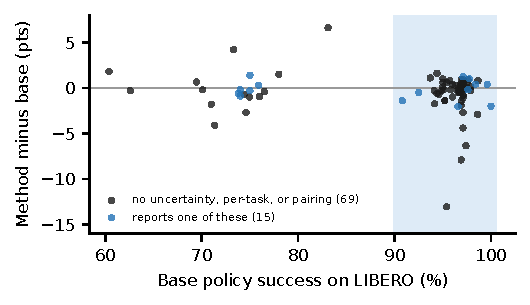
\includegraphics[width=0.92\columnwidth]{figures/fig_efficiency.pdf}
\caption{No-loss claims in the $\NumEffPlotted$ audited VLA efficiency
papers with numeric LIBERO rates: base-policy success vs.\ method minus
base. Shaded: base at or above $90\%$, where Sec.~\ref{sec:dilution}
shows certificates are least informative. Blue: the claim reports
uncertainty, per-task results, or a paired analysis.}
\label{fig:efficiency}
\end{figure}
Following a written search and extraction protocol (one Semantic Scholar
query, logged web and citation searches, and snowballing;
$\NumEffScreened$ candidates screened in two stages), $\NumEffInc$ VLA
inference-efficiency papers claim parity or acceptable loss against their
own base policy on LIBERO (Fig.~\ref{fig:efficiency}). They span step
reduction, distillation, caching, token pruning, quantization, early exit,
and speculative decoding. The base succeeds in at least $90\%$ of episodes
in $\NumEffCeil\%$ of these claims ($\NumEffCeilNf\%$ at $95\%$), and the
median claimed gap is $\NumEffGap$ points. Only $\NumEffAny$ report any
uncertainty, per-task result, or paired analysis for the claim,
$\NumEffPaired$ reports a paired analysis, and $\NumEffNoN\%$ state no
usable episode count. Of the $\NumEffUsable$ claims with counts,
$\NumEffCert$ would certify equivalence at $\pm5$ points from their own
suite averages, and $\NumEffCertRatio$ of those cannot exclude $50\%$ more
failures (Katz interval on the failure-rate ratio). We also checked
whether the same comparisons lose more on harder benchmarks the papers
report; they do not (larger loss in $\NumEffLarger$ of $\NumEffPairs$
papers), though those benchmarks are chosen by the authors and are often
small real-robot tests in which lower latency can itself raise success.
The field's no-loss claims thus sit where certificates are least
informative; the audit does not show that the shortcuts they certify are
costly. Extraction was LLM-assisted; direct text search of a seeded $20\%$
sample confirmed $\NumEffVerAuto$ of $\NumEffVerFields$ extracted fields,
and manual checks the remaining $\NumEffVerMiss$.

\textbf{Other reporting gaps.} In a separate audit of $131$ highlighted
comparisons from 50 VLA papers, $34.4\%$ state no usable rollout count and
evaluation-seed counts appear for $31$; among recomputable comparisons,
$31.4\%$ fail an exact test at the papers' own rollout counts, concordant
with Jiang et al.~\cite{jiang2026benchmarking}. \NumDialSentence

\section{Limitations}\label{sec:limitations}
All results are simulation-only and LIBERO-family, on three
flow-matching policies, two from one model family. The core
demonstration rests on one policy: the equivalence certificates in our
grids come from $\pi_{0.5}$ and share arms, the informative/saturated
classification was made for a different purpose, and the informative
half's evidence rests mostly on one task. We test one acceleration, the
single denoising step; the audit shows the other families make the same
kind of claim but does not re-test them. The ratio bound of $1.5$ is
illustrative. Latency is inference time on one A100. The audits were
single-rater against fixed rules and LLM-assisted over full text; the
efficiency audit's search could not use the arXiv API and its snowballing
was limited to papers flagged during reading. Neither has yet been
checked by a human second rater. All extractions ship with verbatim
evidence.

\section{Conclusion}
A no-loss verdict on a saturated benchmark is valid for the average it
certifies and says little about the tasks on which policies fail. Across
our grids, saturated tasks keep nearly every equivalence certificate and
informative tasks keep almost none, while differences survive where
failures occur; where failures are common, one step costs $\pi_0$
$\NumPiZeroCost$ points and $\pi_{0.5}$ $\NumCameraCost$ points under large
camera shifts. The VLA efficiency literature makes its claims in exactly
this regime. Authors should report discordant pairs, results on
informative tasks, and a relative margin; reviewers should ask for them;
and practitioners should treat ``no loss on LIBERO'' as a claim about
tasks their policy already solves.

\bibliographystyle{IEEEtran}
\bibliography{refs}

\end{document}
